\section{Trace Funktion}\label{Validierung:Trace Funktion}
\begin{itemize}
  \item Beispielprogramme in PEARL definieren
  \item Anforderungen validieren:
  \begin{itemize}
    \item Laufzeiten der einzelnen Programme mit und ohne Trace Funktionalität
    bestimmen und vergleichen, mit Python Programm
    \cref{lst:Python_Benchmark_CPU}
    \item Speicherauslastung der einzelnen Programme mit und ohne Trace
    Funktionalität bestimmen und vergleichen, mit Python Programm
    \cref{lst:Python_Benchmark_Memory}
  \end{itemize}
\end{itemize}

\begin{listing}[ht]
  \inputminted[frame=lines,linenos]{python}{./Python/benchmark_cpu.py}
  \caption{Pythonskipt zur Messung der Laufzeit}
  \label{lst:Python_Benchmark_CPU}   
\end{listing} 

\begin{listing}[ht]
  \inputminted[frame=lines,linenos]{python}{./Python/benchmark_memory.py}
  \caption{Pythonskipt zur Messung der Speicherauslastung}
  \label{lst:Python_Benchmark_Memory}   
\end{listing} 

\section{Analyse Programm}
\label{section:ValidierungAnalyseProgramm}
Für die chronologische Darstellung der Lockobjekte wird die Trace-Datei aus
\cref{lst:ExampleTraceFile} mit drei Threads und neun Lockobjekten.
\begin{listing}[ht]
  \begin{minipage}[ht]{\linewidth}
    \begin{multicols}{3}
      \inputminted[linenos]{text}{./Examples/ExampleTraceFile.log}
    \end{multicols}
    \caption{Beispielhafte Trace-Datei mit einem potenziellen Deadlock}
    \label{lst:ExampleTraceFile}
  \end{minipage}
\end{listing}
In dem Beispiel gibt es zusätzlich zwei Einträge mit dem gleichen Zeitstempel in
den Zeilen 3 und 4 sowie in den Zeilen 13 und 14. Die Ausgabe der Anwendung aus
\cref{section:Implementierung:Analyse Programm} ist in
\cref{fig:LockTraceVisualization} dargestellt.
\begin{figure}[ht]
  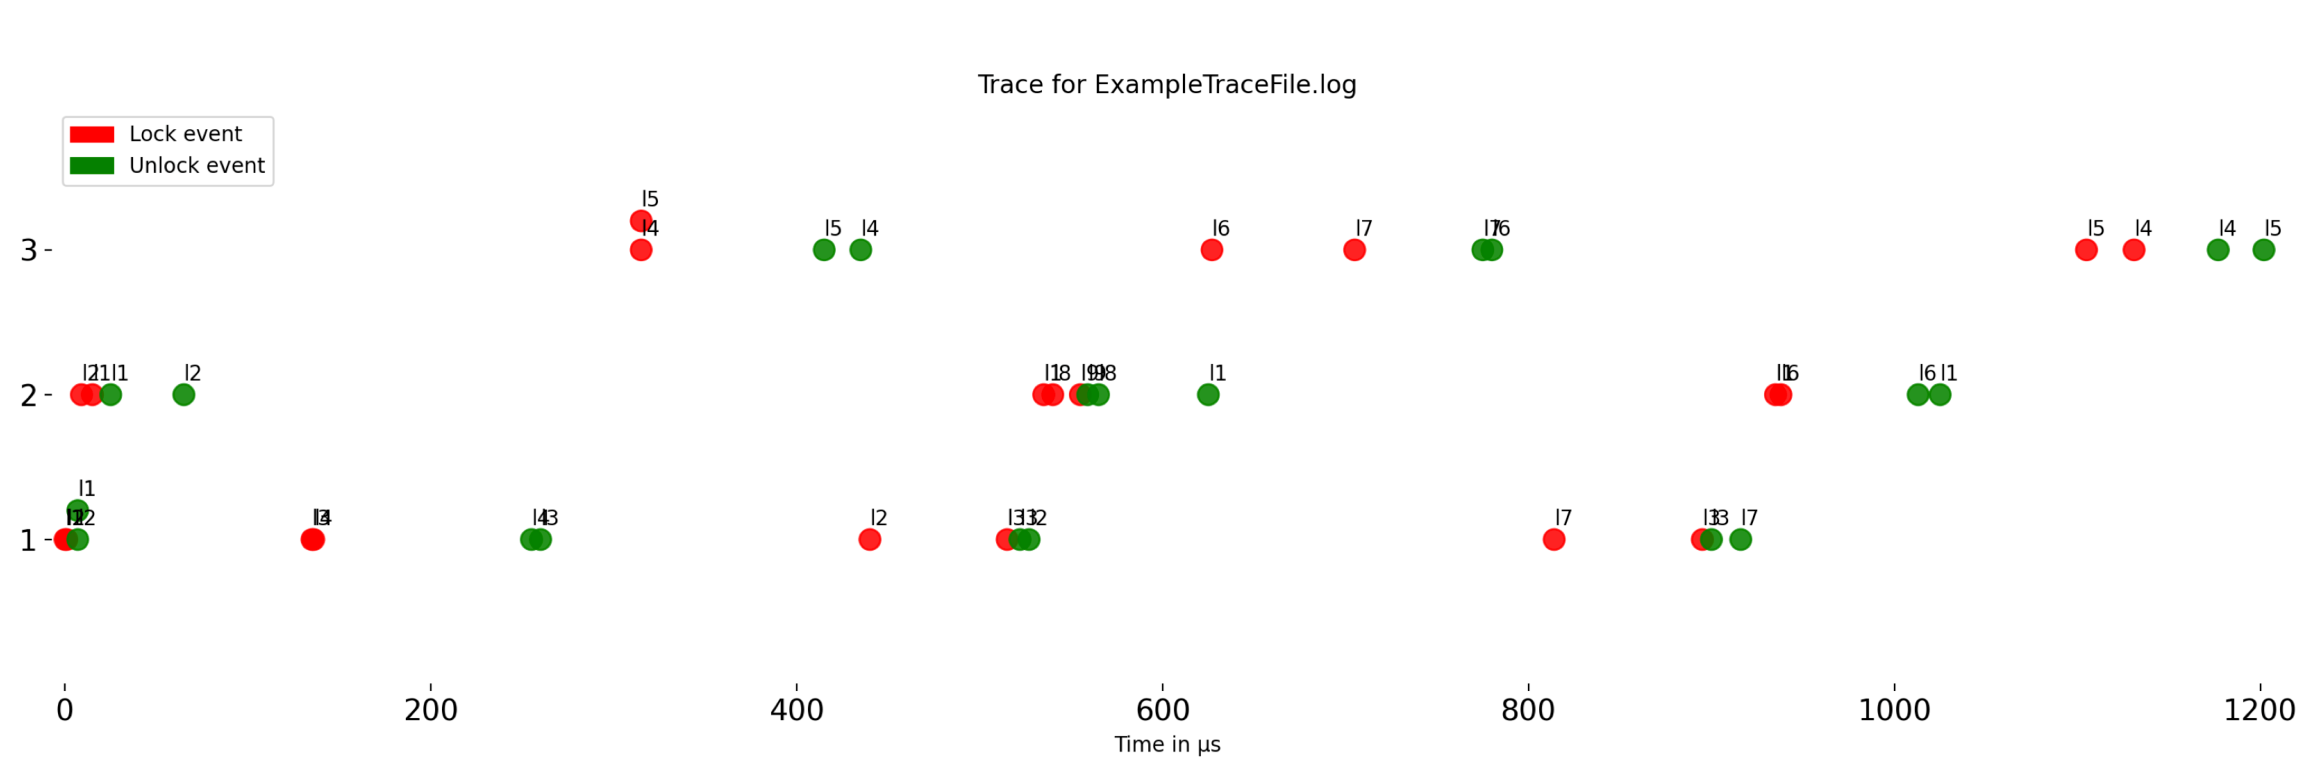
\includegraphics[width=\linewidth]{ExampleTraceFile.eps}
  \caption{Ausgabe der Analyse-Anwendung}
  \label{fig:LockTraceVisualization}
\end{figure}
Die überlappenden Logeinträge können auseinander gezogen werden in dem in den
Graphen hineingezoomt wird. Wird zum Beispiel auf die ersten 70 Mikrosekunden
vergrößert, werden die Logeinträge auseinander gezogen siehe
\cref{fig:LockTraceVisualizationZoomed}.
\begin{figure}[ht]
  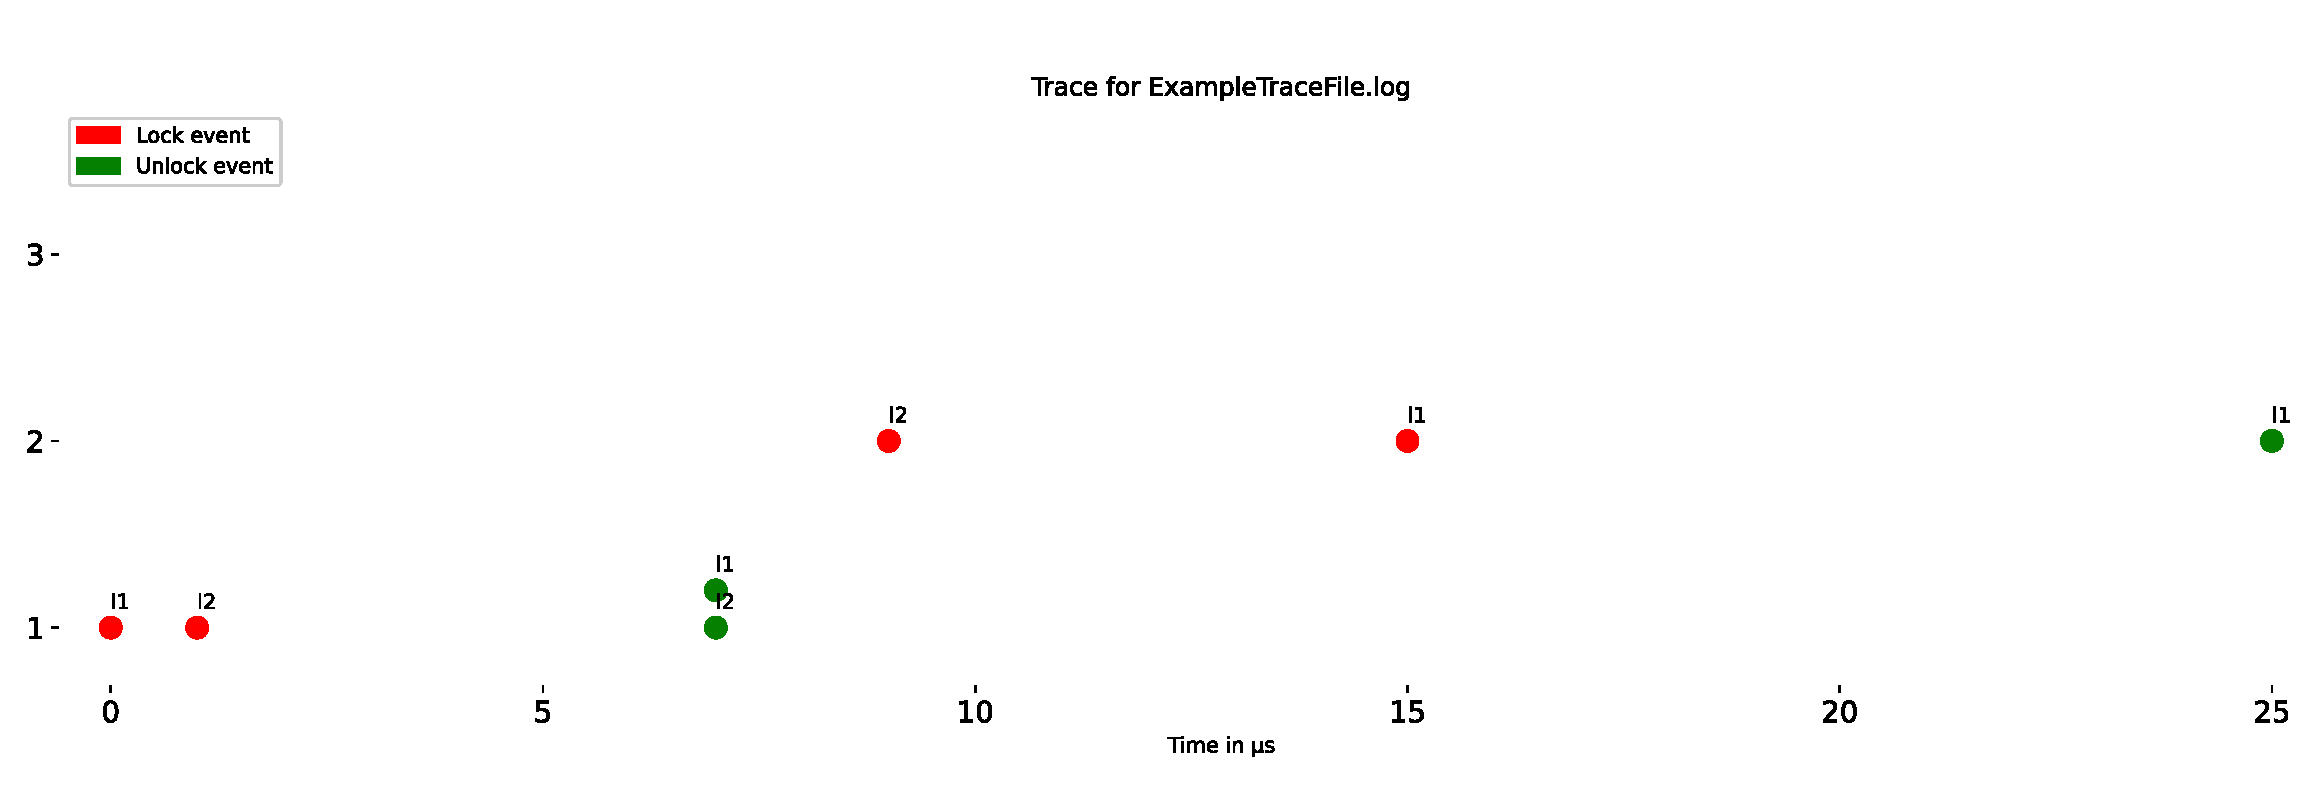
\includegraphics[width=\linewidth]{ExampleTraceFileZoomed.eps}
  \caption{Vergrößerte Darstellung von \cref{fig:LockTraceVisualization}}
  \label{fig:LockTraceVisualizationZoomed}
\end{figure}
Die beiden Logeinträge mit den gleichen Zeitstempel sind bei 7 Mikrosekunden
korrekt vertikal versetzt dargestellt.


\section{Visualisierung von potenziellen Deadlocks}
\label{section:DeadlockVisualization}
Für die Visualisierung von potenziellen Deadlocks wird wieder die Trace-Datei
aus \cref{lst:ExampleTraceFile} verwendet. In dem Beispiel gibt es genau einen
potenziellen Deadlock zwischen den Threads \textit{1} und \textit{2}. In den
Zeilen 1 und 2 nimmt der Thread \textit{1} die Lockobjekten \textit{l1} und
\textit{l2} nacheinander in Besitz. In den Zeilen 5 und 6 nimmt der Thread
\textit{2} die Lockobjekte \textit{l2} und \textit{l1} nacheinander in Besitz.
Der potenzielle Deadlock entsteht, da der Thread \textit{1} zuerst das
Lockobjekt \textit{l1} in Besitz nehmen kann und bevor dieser das Lockobjekt
\textit{l2} in Besitz nehmen kann, kann der Thread \textit{2} das Lockobjekt
\textit{l2} bereits in seinen Besitz genommen haben. Dadurch blockieren sich
beide Threads gegenseitig und ein Deadlock entsteht. Die Ausgabe der Anwendung
zur Erkennung und Visualisierung von potenziellen Deadlocks ist in
\cref{fig:DeadlockVisualization} dargestellt.
\begin{figure}[ht]
  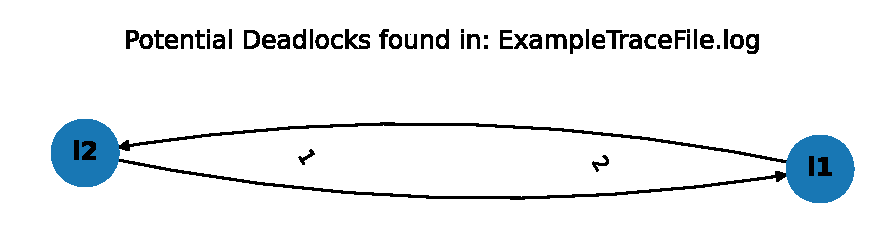
\includegraphics[width=\linewidth]{ExamplePotentialDeadlocks.eps}
  \caption{Ergebnis der Erkennung von potenziellen Deadlocks aus \cref{lst:ExampleTraceFile}}
  \label{fig:DeadlockVisualization}
\end{figure}
Die Beschriftung der Kanten erfolgt immer zum Ende der Kante hin, zum Beispiel
gehört die Beschriftung \textit{1} zu der Kante von \textit{l1} zu \textit{l2}.
Zusätzlich zur grafischen Darstellung werden die Ergebnisse als
Zyklische-Lock-Dependency-Chain auf der Konsole ausgegeben. Für die verwendete
Trace-Datei wird "(1,l2,{l1}) (2,l1,{l2})" als potenzieller Deadlock auf der
Konsole ausgegeben.